\documentclass[systemskiss/skiss.tex]{subfiles}

\begin{document}
\section{Sensormodul}
Sensormodulen innehåller alla de sensorer som bilen behöver för att kunna mäta avstånd i sin omgivning. Denär direkt kopplad till kommunikationsmodulen via en databuss.
\subsection{Översiktlig beskrivning av modulen}
\begin{figure}[h]
    \centering
    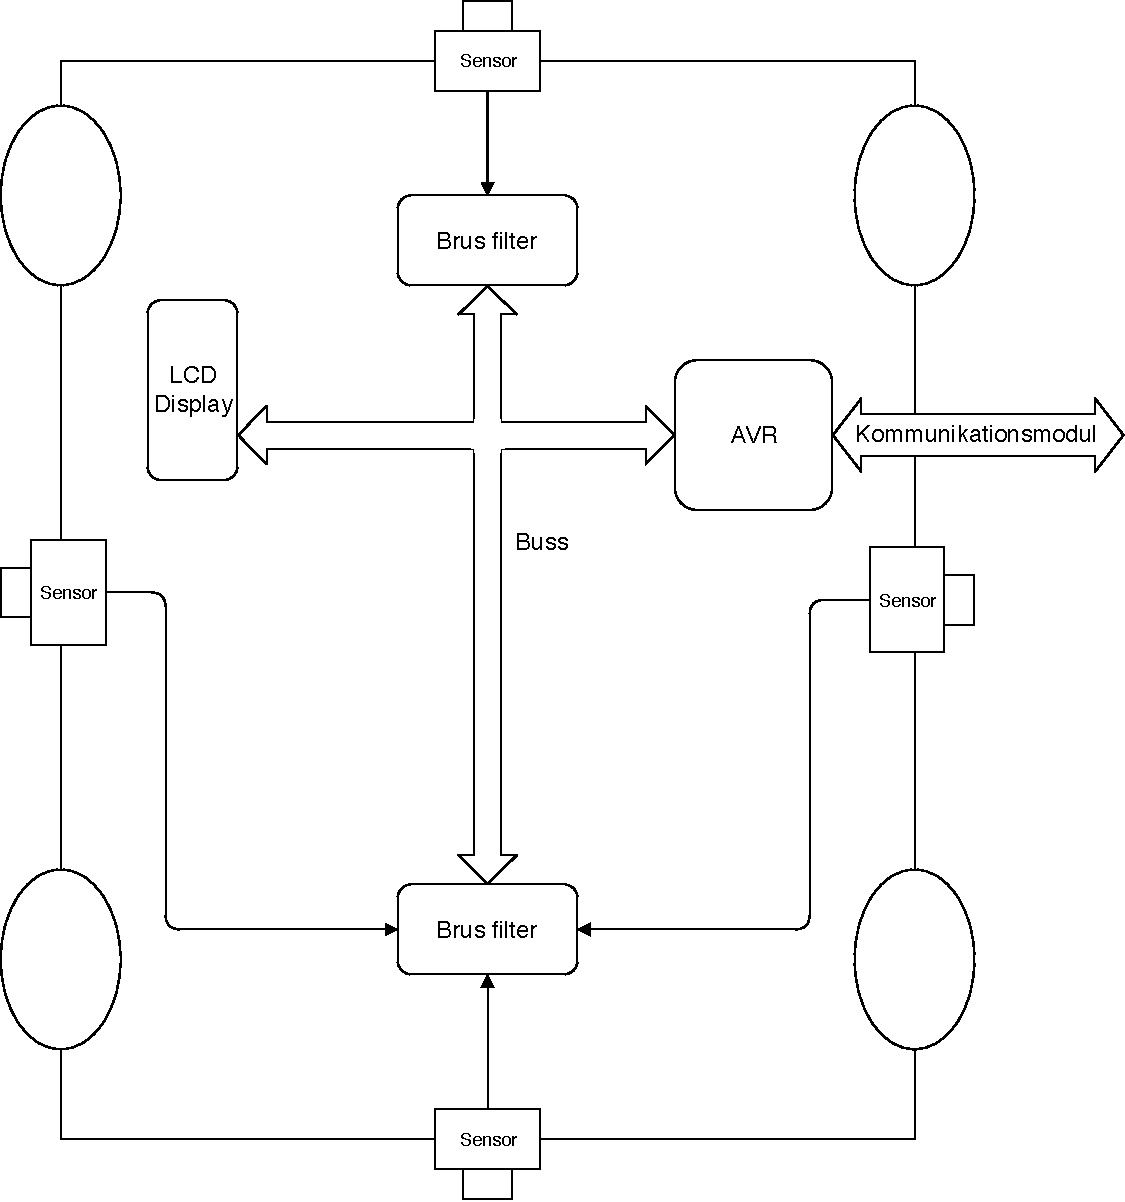
\includegraphics[width=0.6\linewidth]{systemskiss/figures/sensormodul.pdf}
    \caption{Övergripande bild över sensormodulen}
    \label{fig:sensorskiss}
\end{figure}


\end{document}

